\documentclass{presentacion}

\usepackage[utf8]{inputenc}

\hypersetup{pdfpagemode=FullScreen}

\usepackage[spanish]{babel}
\usepackage{listings}
\usepackage[T1]{fontenc}

\usepackage[backend=bibtex,style=alphabetic]{biblatex}
\bibliography{referencias}


\usepackage[newfloat=true]{minted} % syntax highlighting
\usemintedstyle{rainbow_dash}


\usepackage{changepage} % provee adjustwidth

\usepackage{graphicx}
\usepackage{epstopdf}
\epstopdfsetup{update} % only regenerate pdf files when eps file is newer


%\usefonttheme{professionalfonts} % using non standard fonts for beamer
\usefonttheme{structurebold} % using non standard fonts for beamer

\addtobeamertemplate{frametitle}{
   \let\insertframetitle\insertsectionhead}{}
\addtobeamertemplate{frametitle}{
   \let\insertframesubtitle\insertsubsectionhead}{}


\makeatletter
  \CheckCommand*\beamer@checkframetitle{\@ifnextchar\bgroup\beamer@inlineframetitle{}}
  \renewcommand*\beamer@checkframetitle{\global\let\beamer@frametitle\relax\@ifnextchar\bgroup\beamer@inlineframetitle{}}
\makeatother
   
\AtBeginSection[]
{  
  \begin{frame}
    \frametitle{Índice}
    \tableofcontents[currentsection]
  \end{frame}
}

\usebackgroundtemplate%
{%
    \includegraphics[width=\paperwidth,height=\paperheight]{img/}%
}

\title[Virtual Threads] 
{Usando virtual threads para incrementar dramáticamente la paralelización de tu aplicación }
\subtitle{JConf Perú 2023}
\author{Andrés Alcarraz}
\date{Sábado 2º de Diciembre de 2023}

% configuración de tema
\usetheme{Madrid}
%\usetheme{default}
\usecolortheme{seahorse}

\usepackage{worldflags}
\flagsdefault[width=1em, framewidth=0px]

%\addtobeamertemplate{background canvas}{\transuncover}{}

\begin{document}
\frame{\titlepage}

\section{Acerca de mí}
\begin{frame}
    \begin{itemize}
        \item Uruguayo \worldflag{UY}
        \item 24 años desarrollando en Java.
        \item     \email{alcarraz@gmail.com}
        \item \linkedin{andresalcarraz}
        \item \twitter{andresalcarraz}
        \item \github{alcarraz}
        \item \stackoverflow{3444205}
        
    \end{itemize}
\end{frame}

\section{Un poco de historia}

\subsection{Historia de la multitarea en Java}
\begin{frame}
 \begin{itemize}[<+->]
  \item Green threads: Java 1.1. Todos los threads compartían un thread del sistema operativo. \cite{JavadocExecutor}
  \item  Native threads:  Introducidos en java 1.2 (1998)
  \item Executors: Introducidos en Java 5.0 (JEP 444 \cite{JEP444}).
  \begin{itemize}
   \item Thread pools: ya no hay que implementarlos a mano o depender de bibliotecas.
   \item Scheduling.
  \end{itemize}
  \item Programación reactiva, nombre cool, pero lo cool termina ahí.
  \item Java 21: virtual threads, bloquear está bien de nuevo.
  
 \end{itemize}

\end{frame}

\subsection{El problema con los threads nativos}
\begin{frame}
 \begin{itemize}[<+->]
  \item Costosos de crear.
  \item Costosos de mantener.
  \item En llamadas bloqueantes, los recursos quedan bloqueados.
  \item Veamos un ejemplo, ¡Coding time!.
 \end{itemize}
\end{frame}

\subsection{La solución reactiva}

\begin{frame}[fragile]
Ejemplo tomado de José Paumard, que a su vez lo toma de Tomasz   Nurkiewicz. \cite{Java21VritualThreadsVideo}
    \begin{minted}{java}
User user = userService.findUserByName(name);
if (!repo.contains(user)) repo.save(user);

var cart = cartService.loadCartFor(user);
var total = cart.items().stream()
                .mapToInt(Item::price)
                .sum();

var transactionId = paymentService.pay(user, total);
emailService.send(user, cart, transactionId);
     
    \end{minted}

\end{frame}

\begin{frame}[plain,fragile]
\fontsize{7pt}{8pt}\selectfont
 
    \begin{minted}{java}
var future = supplyasync(() -> userService.findUserByName(name))
        .thenCompose(
                user -> allof(
                        supplyAsync(() -> !repo.contains(user))
                        .thenAccept (
                            doesNotContain -> {
                                if (doesNotContain) repo. save(user);
                            }
                        ),
                        supplyAsync(
                            () -> cartservice.loadCartFor(user)
                                .thenapply(
                                    cart ->
                                        supplyAsync(() -> cart.items().stream().mapToInt(Item::price).sum())
                                                .thenapply(
                                                    total -> paymentService.pay(user, total))
                                                    .thenAccept (
                                                        transactionId -> emailService.send(user, cart, transactionId)
                                                    )
                                )
                        )
                )
        )
    \end{minted}
\end{frame}

\begin{frame}
    \begin{itemize}
     \item Operaciones escritas como lambdas
     \item El resultado de una es pasado a la siguiente.
     \item No se debe bloquear en las lambdas.
     \begin{itemize}
        \item Cuando se está esperando por un recurso externo, retornar con un future.
     \end{itemize}
     \item Adiós a la programación imperativa.
     \item La lógica de negocio se mezcla con la lógica del framework \textrightarrow complica cambios en la lógica de negocio.
     %\item Stacktrace no es de mucha ayuda al depurar. Contexto del framework no de la aplicación.
     \item Si una lambda, genera un error en el framework, no es trivial descubrir cual fue.
    \end{itemize}
\end{frame}


\section{Propiedades de los Virtual Threads}
\subsection{Ventajas}
\begin{frame}
 \begin{itemize}[<+->]
  \item Solución nativa.
  \item Fáciles de usar.
  \item Livianos.
  \item Código legible.
  \item No se necesita hacer pool de ellos.
  \item Revisitemos el ejemplo anterior.
 \end{itemize}

\end{frame}

\subsection{Desventajas}
\begin{frame}
 \begin{itemize}[<+->]
  \item No hay una solución nativa para limitar el número de threads.
  \item Por lo tanto no hay una forma trivial de limitar el acceso a un recurso.
  \item Usar semáforos para controlar esto.
  \item Se puede crear un executor personalizado para esto.
 \end{itemize}
\end{frame}

\subsection{Como se usan}
\begin{frame}[fragile]
    \begin{itemize}
        \item Factory method en la clase \mintinline{java}{Thread}
        \begin{minted}{java}
Thread virtual = Thread.ofVirtual().start(
  () -> System.out.println("Hola Mundo!"));
        \end{minted}
        \item Con executors:
        \begin{minted}{java}
ExecutorService service 
  = Executors.newVirtualThreadPerTaskExecutor();
...
service.execute( 
  () -> System.out.println("Hola Mundo!"));
        \end{minted}
        \item Por cierto, \mintinline{java}{ExecutorService} ahora implementa \mintinline{java}{AutoCloseable}.
        ¡Se puede utilizar en try-with-resources!
    \end{itemize}
\end{frame}



\subsection{Que hacer}
\begin{frame}
 \begin{itemize}[<+->]
  \item Bloquear está bien, ¡para eso están!
  \item Usarlos para tareas intensivas en el uso de recursos externos.
  \begin{itemize}
   \item Operaciones en bases de datos.
   \item Llamadas a servicios REST.
   
  \end{itemize}

 \end{itemize}
\end{frame}

\subsection{Que no hacer}
\begin{frame}
 \begin{itemize}[<+->]
    \item No usarlos para tareas que sólo hagan computación en memoria.
    \item No usarlos para ejecutar parallel streams.
    \begin{itemize}
        \item No deberíamos ejecutar código bloqueante en parallel streams.
    \end{itemize}
    \item Evitar fijar el virtual thread a un platform thread por mucho tiempo.
    \begin{itemize}
        \item No llamar a código nativo que pueda bloquearse.
        \item No usar bloques \mintinline{java}{synchronized} para sincronizar cosas que pueden demorar.
       
             Usar \mintinline{java}{ReentrantLock} en su lugar
    \end{itemize}

 \end{itemize}
\end{frame}

\section{Detalles de implementación}
\begin{frame}
    \begin{center}
        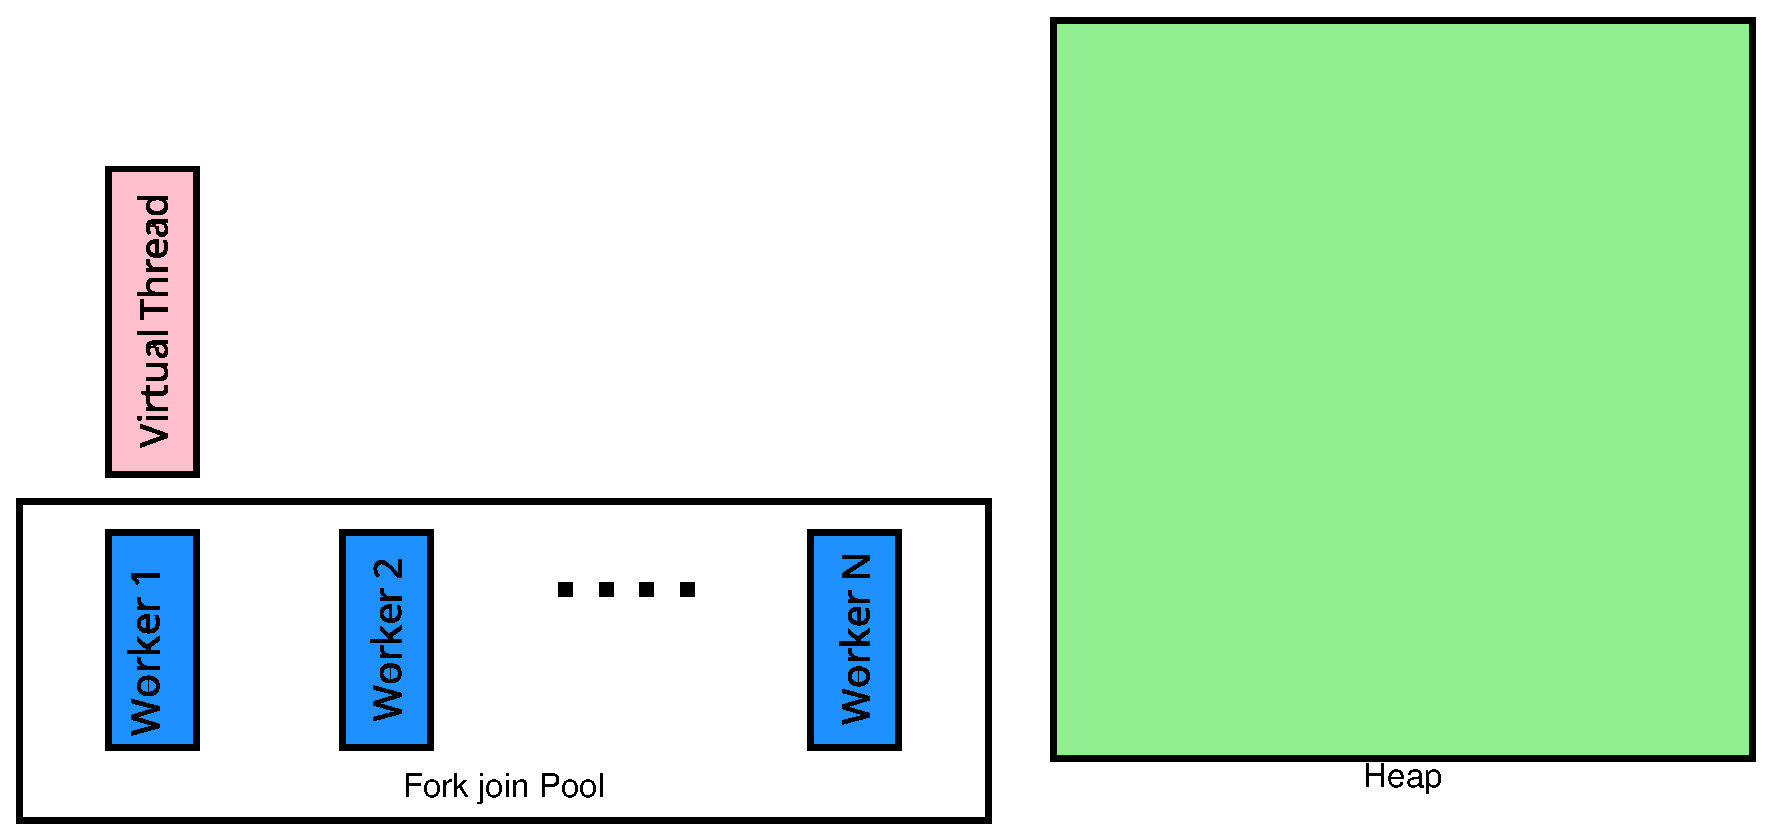
\includegraphics[width=.8\textwidth]{img/implementacion1}
    \end{center}
\end{frame}
\begin{frame}
    \begin{center}
        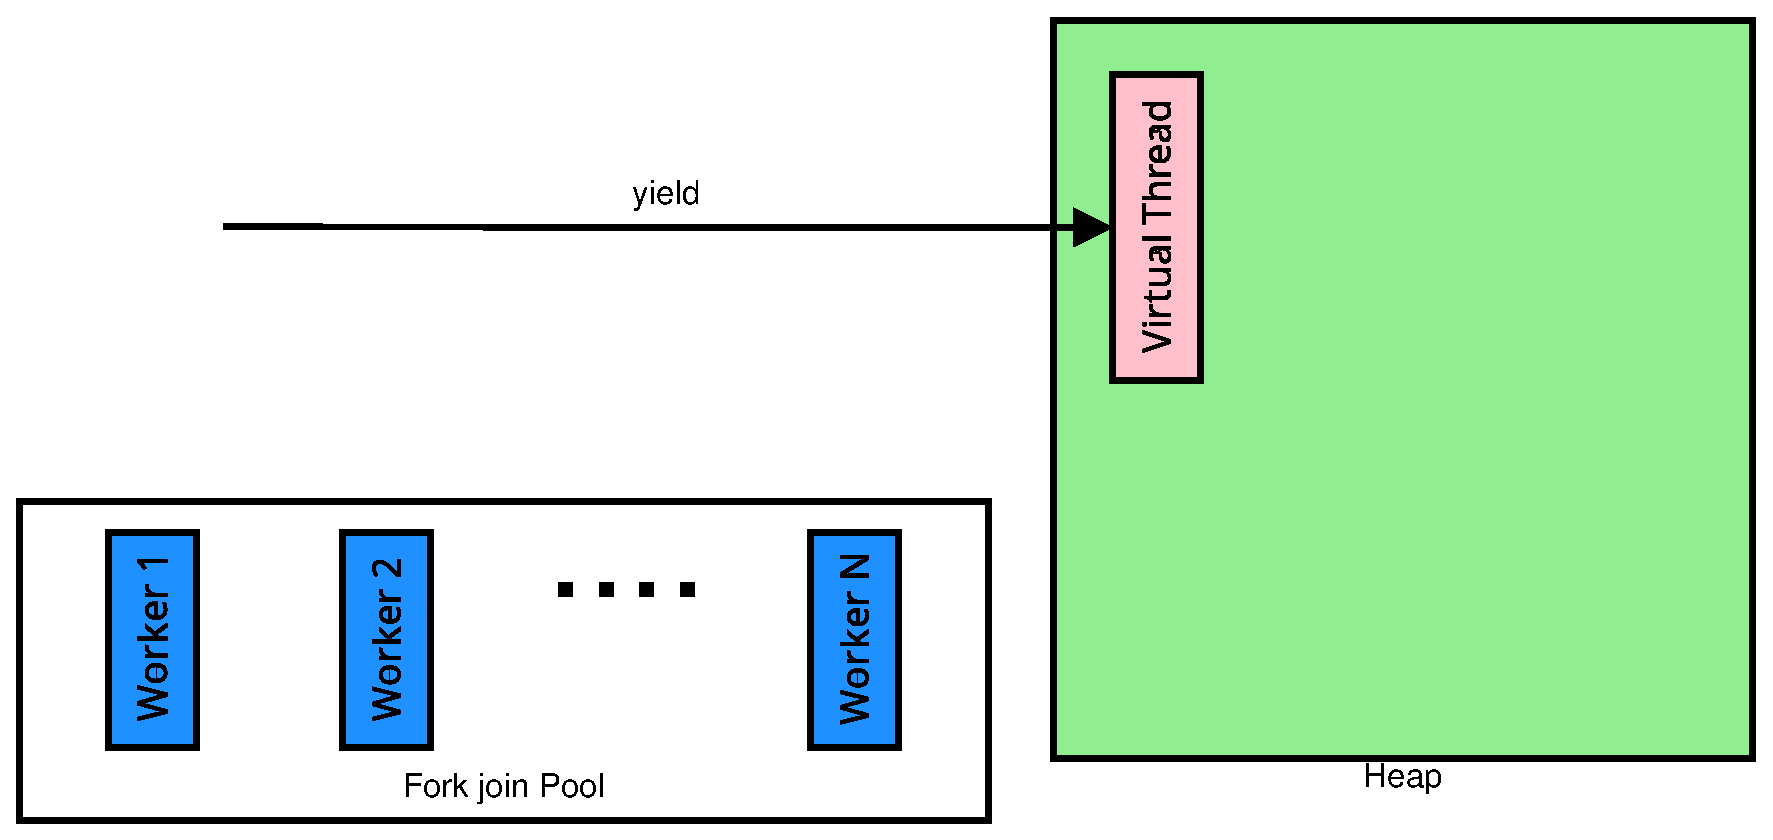
\includegraphics[width=.8\textwidth]{img/implementacion2}
    \end{center}
\end{frame}
\begin{frame}
    \begin{center}
        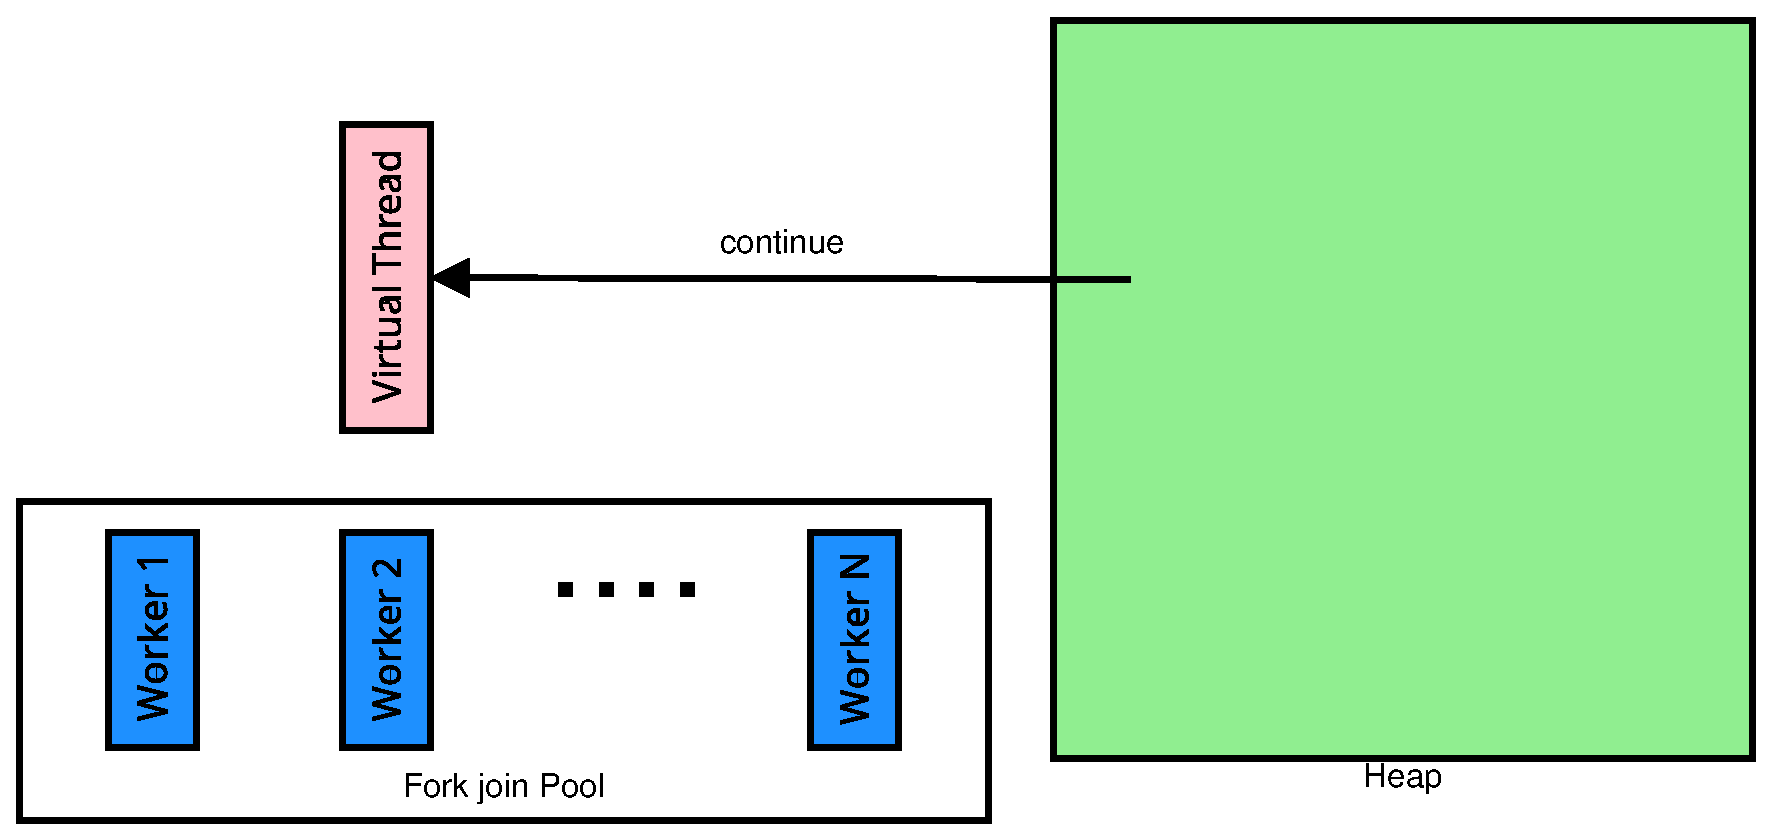
\includegraphics[width=.8\textwidth]{img/implementacion3}
    \end{center}
\end{frame}

\subsection{Pull request}
\begin{frame}
    Se refactorizó todo el código bloqueante de la JDK, para llamar a \mintinline{java}{Continuations.yield()}
    \newline
    \newline
    \includegraphics[width=0.8\textwidth]{img/virtual-threads-PR.png}
\end{frame}

\subsection{\mintinline{java}{Thread.sleep}}
\begin{frame}[fragile,plain]
    \begin{minted}{java}
public static void sleep(long millis) throws InterruptedException {
    if (millis < 0) {
        throw new IllegalArgumentException("timeout value is negative");
    }
    long nanos = MILLISECONDS.toNanos(millis);
    ThreadSleepEvent event = beforeSleep(nanos);
    try {
        if (currentThread() instanceof VirtualThread vthread) {
            vthread.sleepNanos(nanos);
        } else {
            sleep0(nanos);
        }
    } finally {
        afterSleep(event);
    }
}
    \end{minted}
%\end{adjustwidth}
\end{frame}

\section{Frameworks}
\begin{frame}[fragile]
    Probablemente no tengas que escribir código para hacer uso de los virtual threads:
    \vspace{2em}
    \begin{itemize}
     \item Spring: \mintinline{properties}{spring.threads.virtual.enabled=true}
     \item Quarkus: \mintinline{java}{@RunOnVirtualThread}
    \end{itemize}
\end{frame}

\section{Más de project Loom}
\begin{frame}
    \begin{itemize}
        \item Structured Concurrency (Preview) \link{https://openjdk.org/jeps/453}{JEP 453}
        \item Scoped Values (Preview)  \link{https://openjdk.org/jeps/446}{JEP 446}\hspace{1em}(\link{https://openjdk.org/jeps/464}{second preview en Java 22: JEP 464})
    \end{itemize}

\end{frame}

\section{Ejemplo}
\begin{frame}
    \centering
    \textbf{\Huge{Coding time!} }
\end{frame}



%t: top aligned, allowframebreaks para crear automáticamente nuevas páginas de ser necesario
\begin{frame}[t, allowframebreaks]
\frametitle{Referencias}
\printbibliography
\end{frame}


\end{document}
